\documentclass[12pt,a4paper]{report}
% \usepackage[english]{babel}
% \usepackage[utf8x]{inputenc}

\usepackage{graphicx} % Required for inserting images.
\usepackage[margin=25mm]{geometry}
% \renewcommand{\baselinestretch}{1.5}  % Uncomment for 1.5 spacing between lines.
\usepackage[font=sf]{caption} % Changes font of captions.
\usepackage{caption}
\usepackage{subcaption}
\usepackage{float}
\usepackage{amsmath}
\usepackage{amsfonts}
\usepackage{pdflscape}

\title{Reinforcement Learning: CW1}
\author{Haotian Wu (01864103)}

\begin{document}
\maketitle

Note that the 
\section*{Q1: Dynamic programming}
\subsection*{1}
Policy Iteration was used here - policy iteration was chosen as 
it is in general faster.
A small tolerance ($tolerance = 0.00001$) was set for the 
stopping condition of the policy evaluation step. This 
tolerance was chosen to be small enough as to confirm convergence 
of the policy evaluation. Especially as the rewards are to the 
nearest integer the tolerance is sufficiently small.

The Policy Iteration implementation is split into two
stages: the policy evaluation and the policy improvement stages.
Both of these are wrapped in a while loop that only terminates 
when the policy improvement stage does not update the policy 
(the flag $policy_stable$ is set to false if the policy is updated
in policy improvement; otherwise is true and will terminate).

For the policy evaluation, $\Delta$ is initialised to $10 * \theta$ 
where $\theta = tolerance$. This ensures that the policy evaluation
loop will be entered. 
There is a nested loop in Policy Evaluation, the outer one for looping 
through all available states and the inner for updating the value 
for the selected state, ie $V(s)$.
The optimal policy given a state for the current iteration $\pi(s)$,
is computed simply by finding the index with the largest value
in the policy matrix corresponding to state.
The current $V$ is cached as each state requires the original
$V(s')$ to be able update the current $V(s)$.
$P^{\pi(s)}_{s s'}$ is the value from the transition matrix. 
The reward $R^{\pi(s)}_{s s'}$ is also computed given $\pi(s)$.
% This ensures that only the chosen action has a non zero probility
% (note that the policy is greedy, so only one value in the policy should 
% be $1$). Note that the policy is initialised to such that each state
% starts with bias towards the value

The optimal policy (action) is determined for each state

% TODO: finish this section

\subsection*{2}
\begin{figure}[H]
    \centering
    \begin{subfigure}[b]{0.49\textwidth}
        \centering
        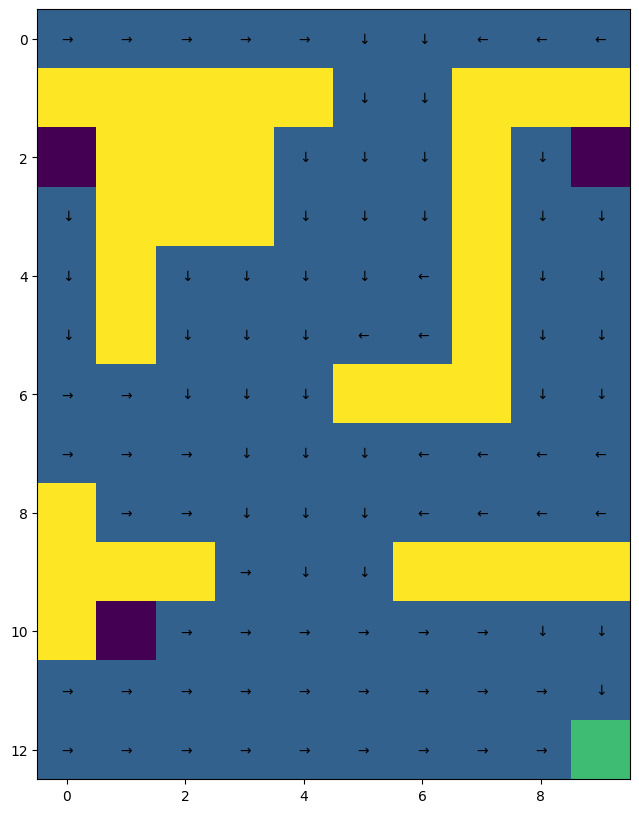
\includegraphics[width=\textwidth]{assets/dp/dp_optimal_policy.png}        
        \caption{Dynamic Programming Policy}
    \end{subfigure}
    \hfill 
    \begin{subfigure}[b]{0.49\textwidth}
        \centering
        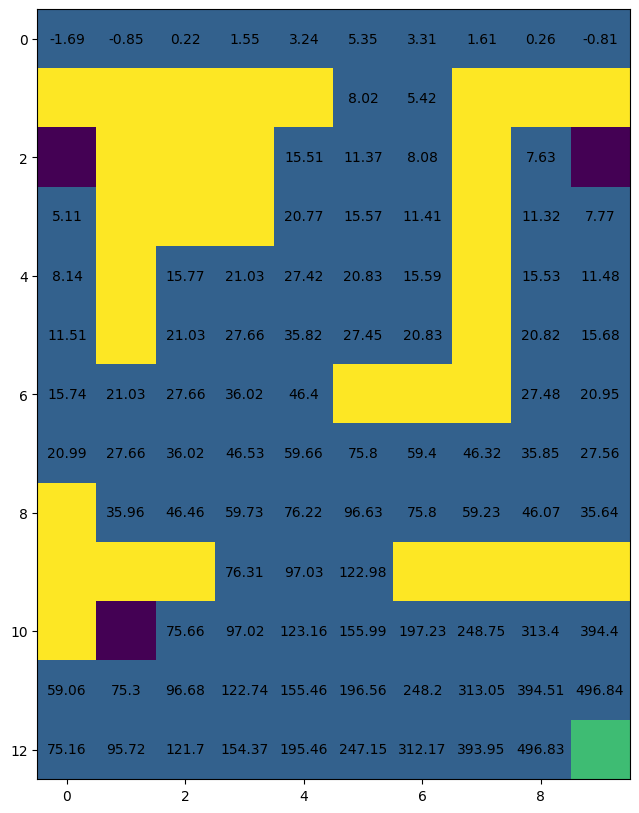
\includegraphics[width=\textwidth]{assets/dp/dp_value_function.png}        
        \caption{Dynamic Programming Value FUnction}
    \end{subfigure}
    \caption*{Graphical Representations of Dynamic Programming Results}
\end{figure} 

\break

\begin{landscape}
\subsection*{3}
\begin{center}
    \begin{tabular}{c || c  c  c}
        & & $\gamma$ & \\
        & 0.1 & 0.25 & 0.5 \\
        \hline \hline \\
        0.2 & 
            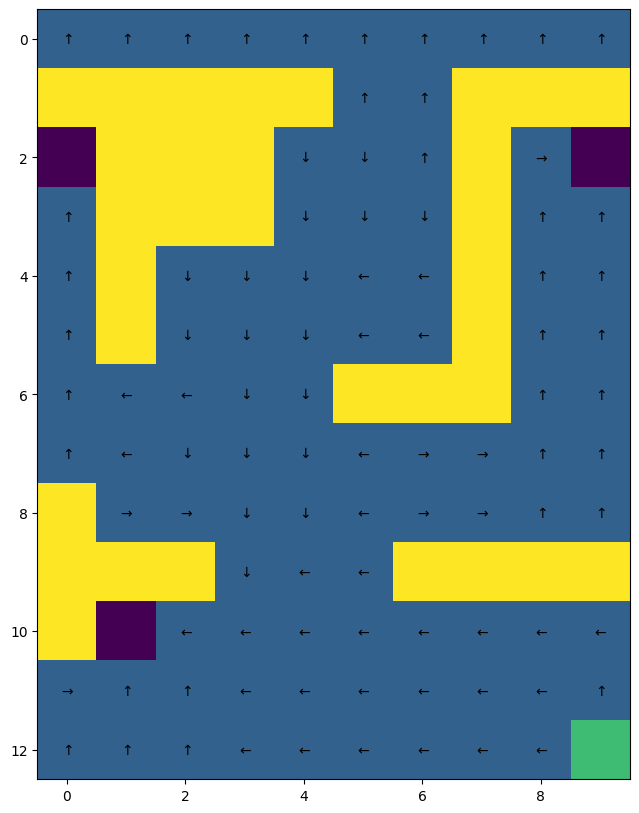
\includegraphics[width=0.35\textheight]{assets/dp/analysis/prob_0.1_gamma_0.2_policy.png}
        & 
            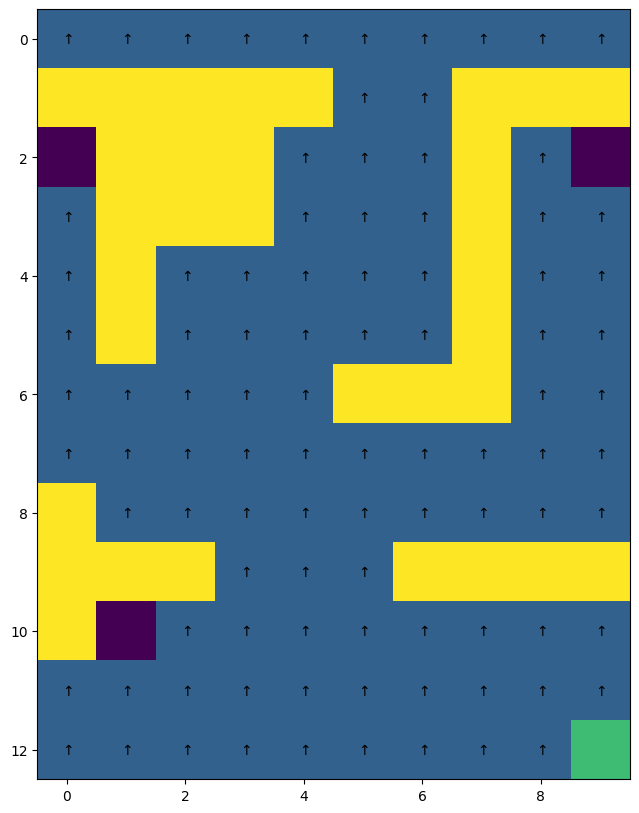
\includegraphics[width=0.35\textheight]{assets/dp/analysis/prob_0.25_gamma_0.2_policy.png}
        & 
            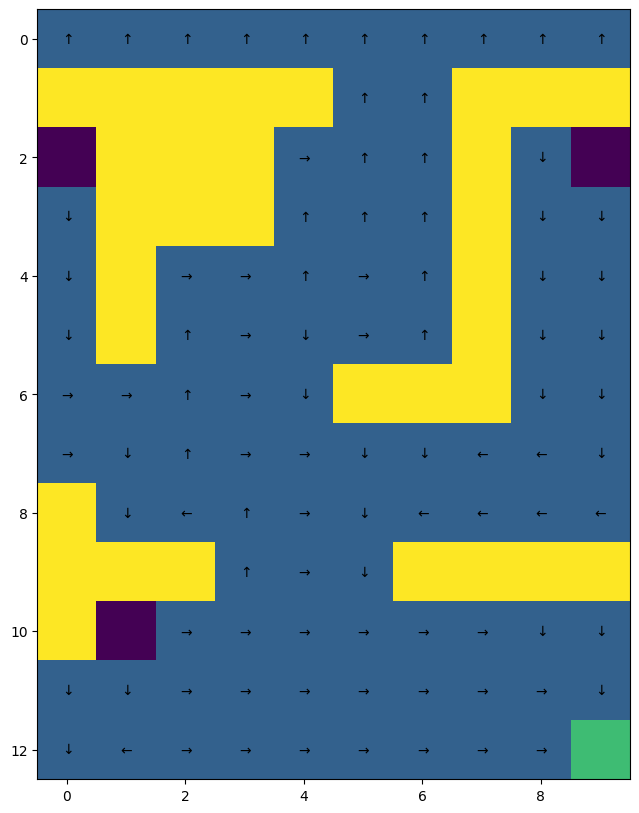
\includegraphics[width=0.35\textheight]{assets/dp/analysis/prob_0.5_gamma_0.2_policy.png}
        \\
        0.8 &
            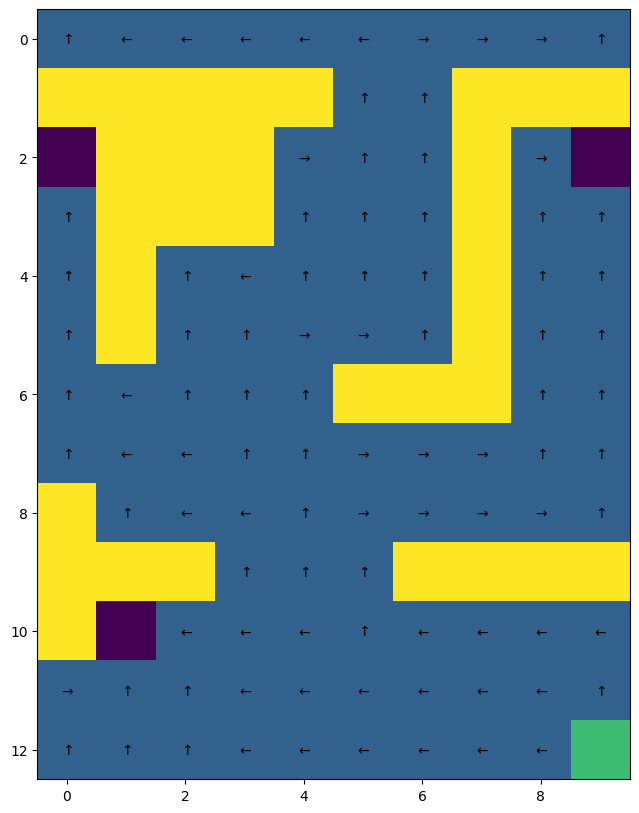
\includegraphics[width=0.35\textheight]{assets/dp/analysis/prob_0.1_gamma_0.8_policy.png}
        & 
            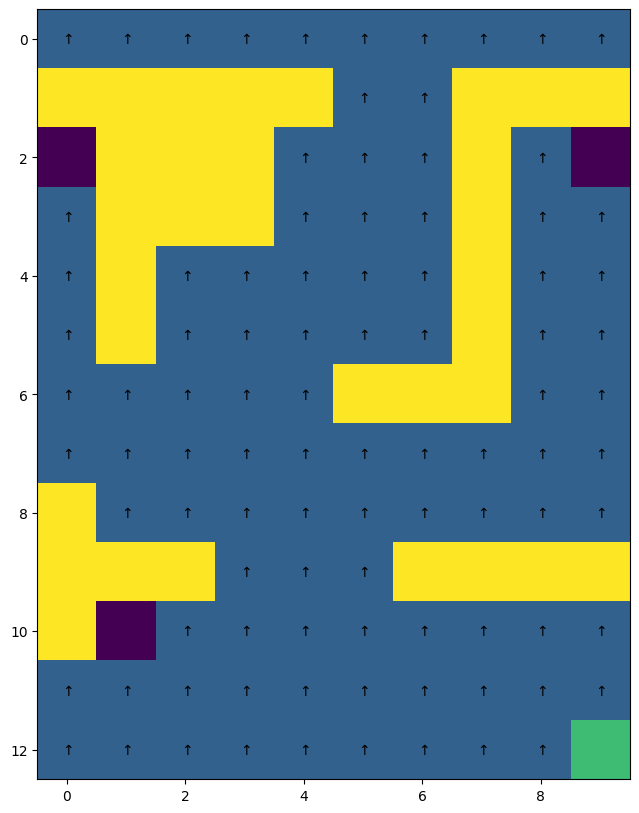
\includegraphics[width=0.35\textheight]{assets/dp/analysis/prob_0.25_gamma_0.8_policy.png}
        &
            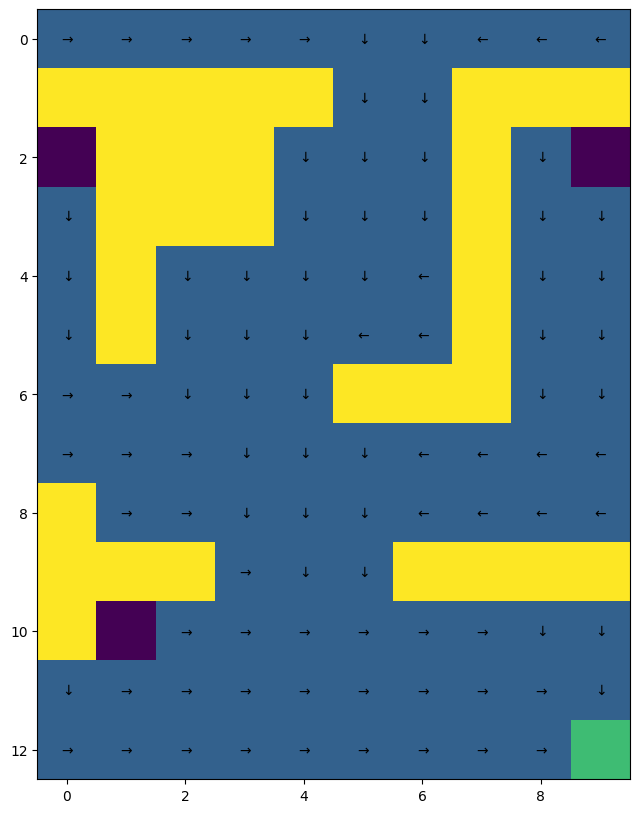
\includegraphics[width=0.35\textheight]{assets/dp/analysis/prob_0.5_gamma_0.8_policy.png}
    \end{tabular}        
\end{center}

\begin{center}
    \begin{tabular}{c || c  c  c}
        & & $\gamma$ & \\
        & 0.1 & 0.25 & 0.5 \\
        \hline \hline \\
        0.2 & 
            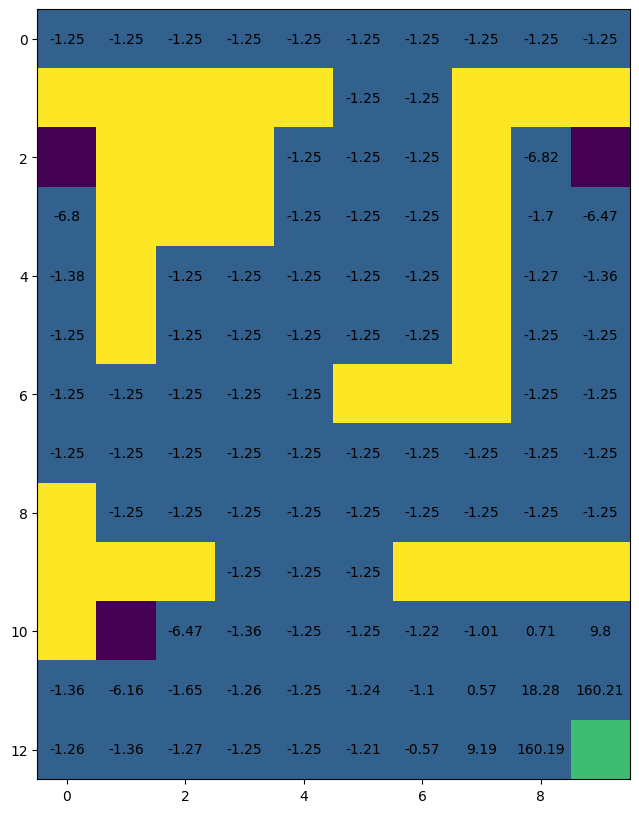
\includegraphics[width=0.35\textheight]{assets/dp/analysis/prob_0.1_gamma_0.2_value.png}
        & 
            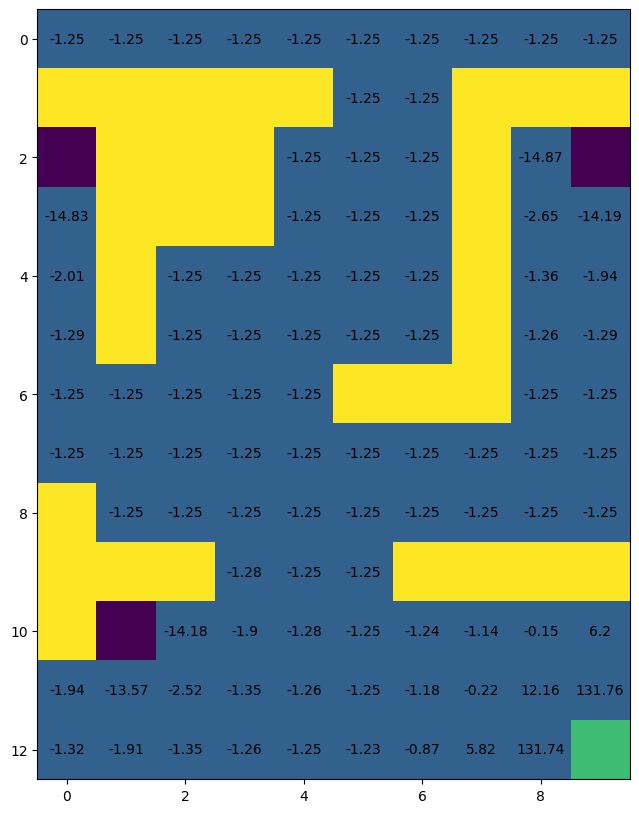
\includegraphics[width=0.35\textheight]{assets/dp/analysis/prob_0.25_gamma_0.2_value.png}
        & 
            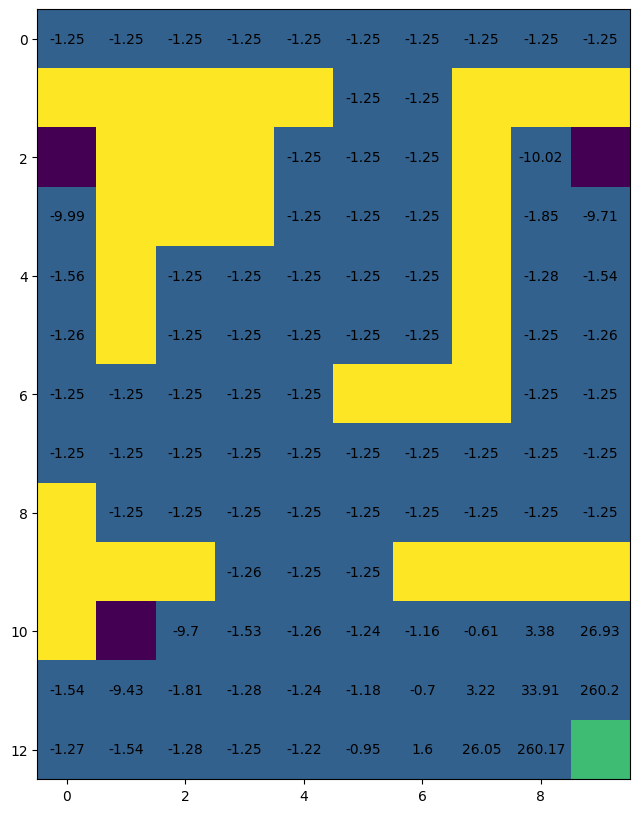
\includegraphics[width=0.35\textheight]{assets/dp/analysis/prob_0.5_gamma_0.2_value.png}
        \\
        \centering 0.8 &
            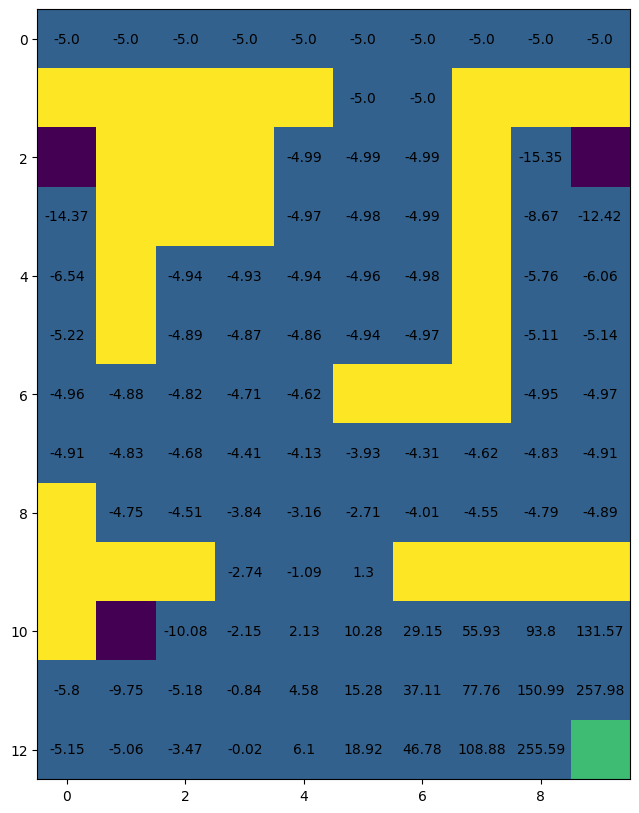
\includegraphics[width=0.35\textheight]{assets/dp/analysis/prob_0.1_gamma_0.8_value.png}
        & 
            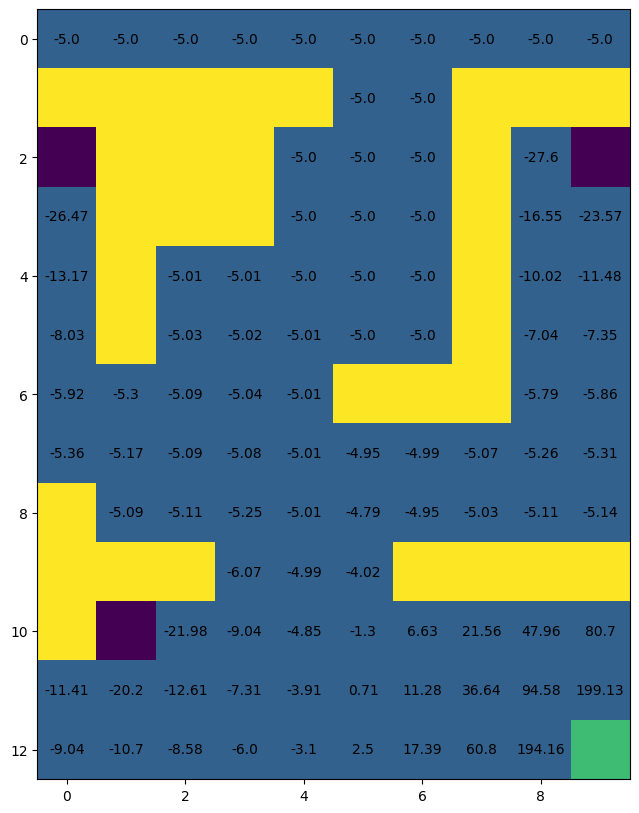
\includegraphics[width=0.35\textheight]{assets/dp/analysis/prob_0.25_gamma_0.8_value.png}
        &
            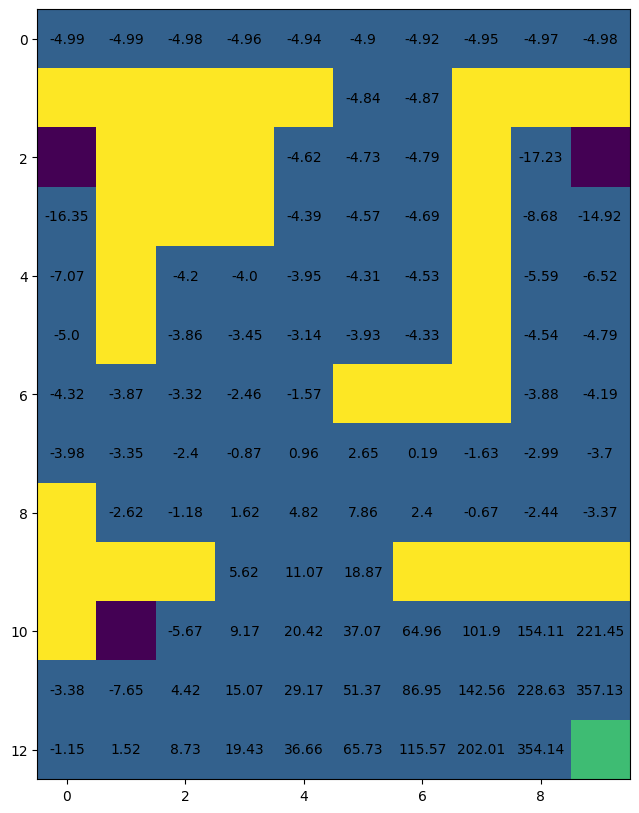
\includegraphics[width=0.35\textheight]{assets/dp/analysis/prob_0.5_gamma_0.8_value.png}
    \end{tabular}        
\end{center}
\end{landscape}
\break

When the probability $p = 0.25$, the transition matrix probability
of success is $0.25$ and the probability of going in another direction
is also $0.25$. 
This results in moving in another direction the same probability 
as the current optimal policy. Consider the policy update $\pi(s) \leftarrow
argmax_a \sum_{s'} P^a_{ss'}[R^a_{ss'} + \gamma V(s')]$: the value $P^a_{ss'}$ 
will be biggest when the 
% TODO
(When $p < 0.25$ this effect is exaggerated and the expected policy 
is not achieved.)

\end{document}